% Phase E draft (docs/10_noisy_label_plan.md). Target: TMLR or a workshop (the
% pre-registered Phase C' rule sent this to a "reframing" write-up).
% Plain article class so it builds anywhere; swap in tmlr.sty / the workshop
% style at submission time. Build: see README.md in this folder.
\documentclass[11pt]{article}

\usepackage[margin=1in]{geometry}
\usepackage[T1]{fontenc}
\usepackage{lmodern}
\usepackage{microtype}
\usepackage{amsmath,amssymb,amsthm}
\usepackage{booktabs}
\usepackage{multirow}
\usepackage{graphicx}
\usepackage{xcolor}
\usepackage[round]{natbib}
\usepackage[colorlinks=true,linkcolor=blue!50!black,citecolor=blue!50!black,urlcolor=blue!50!black]{hyperref}
\usepackage[capitalize,noabbrev]{cleveref}

\newtheorem{proposition}{Proposition}
\newtheorem{corollary}{Corollary}
\theoremstyle{definition}
\newtheorem{definition}{Definition}
\theoremstyle{remark}
\newtheorem{remark}{Remark}
\newtheorem{observation}{Observation}

\newcommand{\TODO}[1]{\textcolor{red}{[TODO: #1]}}
\newcommand{\sg}{\operatorname{sg}}
\newcommand{\clip}{\operatorname{clip}}
\newcommand{\R}{\mathbb{R}}
\newcommand{\dbase}{\delta_{\mathrm{b}}}
\newcommand{\dceil}{\delta_{\mathrm{c}}}
\newcommand{\sd}[1]{\ensuremath{{\scriptstyle\pm#1}}}

\title{When the Margin Goes Negative:\\
Sample Rejection as a Masked-Softmax Margin under Label Noise}
% Double-blind venues: keep anonymous until camera-ready.
\author{Anonymous authors}
\date{Draft, \today}

\begin{document}
\maketitle

\begin{abstract}
Small-loss sample selection, the core heuristic of learning with noisy labels, stops training on
examples the model currently fits poorly. We show that in the masked-softmax family of AS-Softmax
this heuristic is a margin. A sample's loss and gradient vanish exactly when its label gap
$g = \max_{j\neq y} p_j - p_y$ satisfies $g \le -\delta$, so a \emph{negative} per-sample margin
$\delta$ rejects the sample, and every selection rule is a choice of margin function. The view
turns the rule's suspicion statistic into the object of design and yields testable predictions.
A batch-relative statistic is invariant to the batch's overall fit, so the share it rejects cannot
follow the noise rate. An absolute statistic (``another class beats the label'') rejects a
closed-form band of gaps that does not depend on the noise rate, and leaves an escape region of
confidently contradicted labels that no margin in the family can reject. We test these predictions
in a pre-registered study: BERT-base on 20~Newsgroups, six synthetic noise conditions, five seeds,
model selection on noisy held-out labels. The batch-relative margin ties the best robust loss at
40\% symmetric noise but loses 3.8 points on clean data and 4.6 under pair-flip noise, as its
noise-blindness predicts. The absolute margin memorizes the fewest corrupted labels in four of the
five noisy conditions (8--10\% under symmetric noise, against 13--29\% for small-loss selection
given the true noise rate) and is the best method under 40\% pair-flip noise (+5.4 points over
cross-entropy, +3.3 over oracle small-loss). It still trails GCE by 0.9--1.3 points on clean and symmetric noise, so
it fails our pre-registered bar for a new method. Instrumented re-runs locate the costs. A rejected
clean sample receives no gradient and stays locked out (23\% of a noise-free training set under the
batch-relative margin). AS-Softmax, the base loss, initially concentrates its gradient on
mislabeled samples and memorizes them faster than cross-entropy. We report the result as a unifying
view with measured consequences, not as a state-of-the-art method.
\end{abstract}

\section{Introduction}
\label{sec:intro}

Deep networks fit corrupted labels as readily as clean ones \citep{zhang2017understanding}, but
they fit the clean ones first \citep{arpit2017closer,liu2020elr}. Two families of methods exploit
this gap. \emph{Robust losses} such as MAE \citep{ghosh2017robust}, GCE \citep{zhang2018gce} and
SCE \citep{wang2019sce} bound the influence any single example can have on training. \emph{Sample selection} methods
such as MentorNet \citep{jiang2018mentornet}, Co-teaching \citep{han2018coteaching} and DivideMix
\citep{li2020dividemix} drop the examples the model currently fits worst, the \emph{small-loss} trick.
Selection is usually a procedure bolted onto the loss: rank the batch by loss, keep a fraction
$1-r$, and set $r$ from an estimate of the noise rate, often its true value.

This paper starts from an observation about a different line of work. AS-Softmax \citep{lv2023assoftmax}
trains with cross-entropy over a \emph{masked} softmax: a competing class $j$ is dropped from the
normalizer once the label beats it by a margin $\delta$ in probability, $p_y - p_j \ge \delta$. When
every competitor is dropped, the sample's loss and gradient are exactly zero. AS-Softmax uses
$\delta > 0$, so this happens only for samples the model already fits. Nothing in the mechanism
requires $\delta > 0$, however. With $\delta < 0$ the same zero-loss region extends to samples
whose label is \emph{losing}, by up to $|\delta|$. A negative margin is therefore sample
rejection (\cref{prop:zero}), and any selection rule, small-loss included, can be written as a
per-sample margin function (\cref{cor:selection}).

The equivalence is simple, and its value lies in what it makes measurable. Once selection is a
margin $\delta_i = \dbase - \beta\,(2 s_i - 1)$ driven by a per-sample suspicion statistic $s_i$,
the statistic is the design choice and the margin's geometry predicts behavior before any training:
\begin{itemize}
  \item A \textbf{batch-relative} statistic, such as a z-score of $p_y$ within the batch, is invariant
  to the batch's overall level of fit (\cref{prop:blind}). The fraction it flags cannot follow the
  noise rate. The method then rejects about as much on clean data as on noisy data, and the
  strength $\beta$ acts as a hidden, fixed rejection rate.
  \item An \textbf{absolute} statistic, $s_i = \sigma(g_i/\tau)$ with the label gap
  $g = \max_{j\ne y} p_j - p_y$, rejects a closed-form interval of gaps $[g_{\mathrm{lo}}, g_{\mathrm{hi}}]$
  that depends only on $(\beta,\tau,\dbase)$ (\cref{cor:band}). Nothing in it estimates or
  presumes the noise rate.
  \item Because the margin cannot fall below $\dbase - \beta$, \textbf{no} statistic can reject a
  sample whose label is contradicted by more than $\beta - \dbase$ (\cref{prop:reject}). Such
  samples are trained on against their leading class at full strength, and the same cap explains
  why memorization responds to $\beta$ as a threshold rather than smoothly.
\end{itemize}

We test these predictions in a study whose hypotheses, pass criteria and decision rules were
written down before each phase was run (\cref{sec:setup}). The study fine-tunes BERT-base
\citep{devlin2019bert} on 20~Newsgroups \citep{lang1995newsweeder}. It covers symmetric noise at
0--60\% and pair-flip noise at 20 and 40\%, uses five seeds, and selects the model on held-out
\emph{noisy} labels, since a clean validation set is exactly what a practitioner facing label
noise lacks. The predictions hold. The batch-relative margin has the highest mean accuracy of
fourteen methods at the one condition its fixed strength happens to suit, 40\% symmetric noise (a
statistical tie with GCE). It costs 3.8 points on
clean data and fails under pair-flip noise. The absolute margin removes most of the clean-data
cost, memorizes the fewest corrupted labels in four of five noisy conditions and is the most
accurate method under 40\% pair-flip noise. It does \emph{not} match GCE on clean or symmetric
noise, and by our own pre-registered criterion it is not a new state-of-the-art method.

\paragraph{Contributions.}
\begin{enumerate}
  \item An exact equivalence between per-sample margins in masked softmax and sample rejection.
  Small-loss selection, disagreement filtering and AS-Softmax's own sparsity then become points in
  one family of margin functions (\cref{sec:theory}).
  \item Three consequences of the margin geometry: the noise-blindness of batch-relative
  statistics, the rate-free rejection band of the absolute statistic, and an escape region above
  $\beta - \dbase$. Each is verified against the implementation in unit tests.
  \item A pre-registered evaluation with five seeds, a realistic model-selection protocol and a
  tuning grid for the baselines. It reports every pre-registered comparison, including the ones the
  proposed rule loses (\cref{sec:results}). Per-sample gradient instrumentation then locates each
  effect: rejection rates, the clean-data lockout and the escape region (\cref{sec:mechanism}).
  \item Two negative findings: AS-Softmax memorizes corrupted labels \emph{faster} than
  cross-entropy, and estimating the noise rate with a loss mixture, then rejecting, does worse
  here than rejecting disagreement directly.
\end{enumerate}

\section{Background and related work}
\label{sec:background}

\paragraph{Masked softmax.}
Let $o \in \R^C$ be the logits for an input with training label $y$ (possibly corrupted) and
$p = \mathrm{softmax}(o)$. AS-Softmax \citep{lv2023assoftmax} keeps the label and every competitor
the label does not yet beat by a margin $\delta$,
\begin{equation}
  K_\delta = \{y\} \cup \{\, j \ne y : \sg(p_y - p_j) < \delta \,\},
  \qquad
  \ell_\delta(o, y) = -o_y + \log \sum_{j \in K_\delta} e^{o_j},
  \label{eq:masked}
\end{equation}
where $\sg$ is stop-gradient: the mask is recomputed every step but no gradient flows through
it. With $\delta = 1$ the mask keeps every class with $p_j > p_y - 1$, which is all of them
unless $p_y = 1$ exactly, and $\ell_1$ is cross-entropy. AS-Softmax uses a small positive
constant ($\delta = 0.15$ here, reached after a 10\% warm-up). It is one of many margin losses
\citep{liu2016lsoftmax,wang2018amsoftmax,cao2019ldam}. It differs from the angular ones by
working in probability space and by \emph{removing} classes instead of shifting logits, which is
what produces the exact zeros used below.

\paragraph{Sample selection.}
The small-loss trick trains on the fraction of each mini-batch with the lowest loss. The rejected
fraction follows a schedule that ramps to a forget rate $r$, usually set to the true or estimated
noise rate \citep{jiang2018mentornet,han2018coteaching,yu2019coteachingplus,wei2020jocor}.
DivideMix \citep{li2020dividemix}, following \citet{arazo2019unsupervised}, replaces the fixed rate
with a two-component mixture fitted to per-sample losses, and Confident Learning
\citep{northcutt2021confident} estimates per-class noise rates before pruning. A second line filters
on \emph{disagreement} between the prediction and the label: INCV \citep{chen2019understanding} and
SELF \citep{nguyen2020self} keep samples whose (cross-validated or ensembled) prediction matches the
label, SELFIE \citep{song2019selfie} refurbishes labels with consistent predictions, and AUM
\citep{pleiss2020aum} ranks samples by the margin between the assigned logit and the largest other
one, averaged over training. Our absolute statistic is the probability-space, single-step version
of this disagreement signal, applied inside the loss rather than as a separate filtering stage.
Loss truncation \citep{kang2020losstruncation} applies the small-loss idea to text generation.

\paragraph{Selection as an implicit loss.}
Viewing selection as a loss is not new. Self-paced learning \citep{kumar2010spl} selects samples
whose loss is below a threshold, and \citet{meng2017spl} show its alternating optimization
minimizes a concave, robust surrogate of the original loss. Trimmed loss minimization
\citep{shen2019trimmed} and the curriculum loss \citep{lyu2020curriculum} make the same link for
rank-based selection. These views act on the scalar \emph{loss value}. Ours acts inside the
softmax on the \emph{label gap}. The selection threshold then has a direct geometric meaning (how
far another class leads), and the AS-Softmax sparsity, small-loss rejection and disagreement
filtering become one family whose members differ only in the statistic that sets $\delta_i$.

\paragraph{Robust losses and label noise in text.}
Robust losses bound or reshape the gradient of poorly fitted samples instead of zeroing it: MAE
\citep{ghosh2017robust}, GCE \citep{zhang2018gce}, SCE \citep{wang2019sce}, normalized losses
\citep{ma2020normalized}. Others correct the targets \citep{reed2015bootstrap,patrini2017making}
or regularize toward early predictions \citep{liu2020elr}. Surveys cover the field
\citep{song2022survey}, and CIFAR-N provides real human noise for images \citep{wei2022cifarn}.
For text classification, \citet{jindal2019effective} add a noise-modelling layer, and
\citet{zhu2022bert} find pre-trained BERT fairly robust to injected noise when training is stopped
early. Our protocol makes early stopping itself noisy by choosing the epoch on noisy held-out labels.

\section{Rejection as a negative margin}
\label{sec:theory}

Throughout, $g = \max_{j \ne y} p_j - p_y \in (-1, 1)$ is the \emph{label gap}: $g < 0$ when
the training label is the model's top class, and $g > 0$ when some other class beats it. All
statistics below are computed under stop-gradient, as the mask is. Proofs are in
\cref{app:proofs}. Every closed-form number quoted in this section is checked against the code in
\texttt{tests/test\_mechanism.py}.

\subsection{The zero-loss region}

\begin{proposition}[Zero loss $\Leftrightarrow g \le -\delta$]
\label{prop:zero}
For any $\delta \in [-1, 1]$, the masked loss \eqref{eq:masked} satisfies
$\ell_\delta(o, y) = 0 \iff \nabla_o \ell_\delta(o, y) = 0 \iff g \le -\delta$.
If $g > -\delta$, the leading competitor $j^\star = \arg\max_{j\ne y} p_j$ is in $K_\delta$ and
$\ell_\delta > 0$.
\end{proposition}

For $\delta > 0$ this is AS-Softmax's sparsity: a sample stops contributing once its label wins by
at least $\delta$ (\emph{fitted}). For $\delta < 0$ the zero-loss region extends past $g = 0$: a
sample whose label is beaten by up to $|\delta|$ also contributes nothing (\emph{rejected}).
Nothing in the loss distinguishes the two cases. The same exact zero that makes AS-Softmax sparse
is the zero of a discarded sample.

\begin{corollary}[Selection rules are margins]
\label{cor:selection}
Any per-sample keep/reject decision $a_i \in \{0, 1\}$ is realized by $\delta_i = 1$ if $a_i = 1$
and $\delta_i = -1$ otherwise: kept samples train with cross-entropy and rejected ones contribute
nothing. In particular, small-loss selection with forget rate $r$ is the binary margin
$\delta_i = 1 - 2\,\mathbb{1}[\text{sample $i$ is among the $\lceil rB \rceil$ highest-loss samples of
its batch}]$, up to the normalization of the batch mean.
\end{corollary}

\subsection{A family of suspicion margins}

Small-loss uses two margin values. A smooth family interpolates between AS-Softmax and rejection.

\begin{definition}[Suspicion margin]
\label{def:family}
Given a per-sample suspicion statistic $s_i \in (0, 1)$ ($s_i > 1/2$: suspicious), a base margin
$\dbase$, a ceiling $\dceil \ge \dbase$ and a strength $\beta(t) \ge 0$,
\[
  \delta_i = \clip\!\big(\dbase - \beta(t)\,(2 s_i - 1),\; -1,\; \dceil\big).
\]
\end{definition}

We use $\dbase = \dceil = 0.15$, the AS-Softmax value. The ceiling makes the family one-sided: a
confident sample never trains under a tighter margin than AS-Softmax would give it. $\beta(t)$
ramps linearly from 0 to $\beta$ over the first 30\% of training and then holds, the shape of
Co-teaching's forget-rate schedule. $\beta = 0$ is AS-Softmax. We study three statistics:
\begin{itemize}
  \item \textbf{batch-relative} (``M4''): $s_i = \sigma(z_i / T)$ with
  $z_i = (\bar p_y - p_{y,i}) / \mathrm{sd}_B(p_y)$, the z-score of the label probability within
  the mini-batch;
  \item \textbf{absolute gap}: $s_i = \sigma(g_i / \tau)$, suspicious iff another class currently
  beats the label;
  \item \textbf{loss mixture}: the posterior of the high-loss component of a two-component Gaussian
  mixture fitted to per-sample running log-losses, as in DivideMix (\cref{app:mixture}).
\end{itemize}

\begin{proposition}[Rejection condition and the escape region]
\label{prop:reject}
Under \cref{def:family}, sample $i$ has zero loss iff
\[
  g_i \le -\dceil \quad\text{(fitted)} \qquad\text{or}\qquad
  \beta\,(2 s_i - 1) \ \ge\ \dbase + g_i \quad\text{(rejected)}.
\]
Consequently, a sample with $g_i \ge \beta - \dbase$ is never rejected, whatever its statistic,
and trains against at least its leading competitor $j^\star$.
\end{proposition}

The cap $\beta - \dbase$ explains why memorization responds to $\beta$ as a threshold
(\cref{fig:geometry}b). With $\dbase = 0.15$, strengths $\beta = 0.25, 0.5, 1$ can reject only
samples whose label trails by less than $0.10, 0.35, 0.85$. Once early learning has made the model
confident in the true class of a mislabeled sample, its gap is large. A small $\beta$ then rejects
almost none of the noise. At 40\% symmetric noise the three strengths end training with 96\%,
54\% and 16\% of corrupted labels memorized; AS-Softmax ($\beta = 0$) reaches 96\%
(\cref{tab:main}). The escape region also has a cost of its own. A confidently contradicted
label, the clearest case of label noise, then receives a near-maximal per-sample gradient toward
the wrong label. Under the absolute statistic below it is binary cross-entropy against $j^\star$
alone, with $\ell_1$-norm $2(1 - p_y/(p_y + p_{j^\star})) \approx 2$.

\begin{figure}[t]
  \centering
  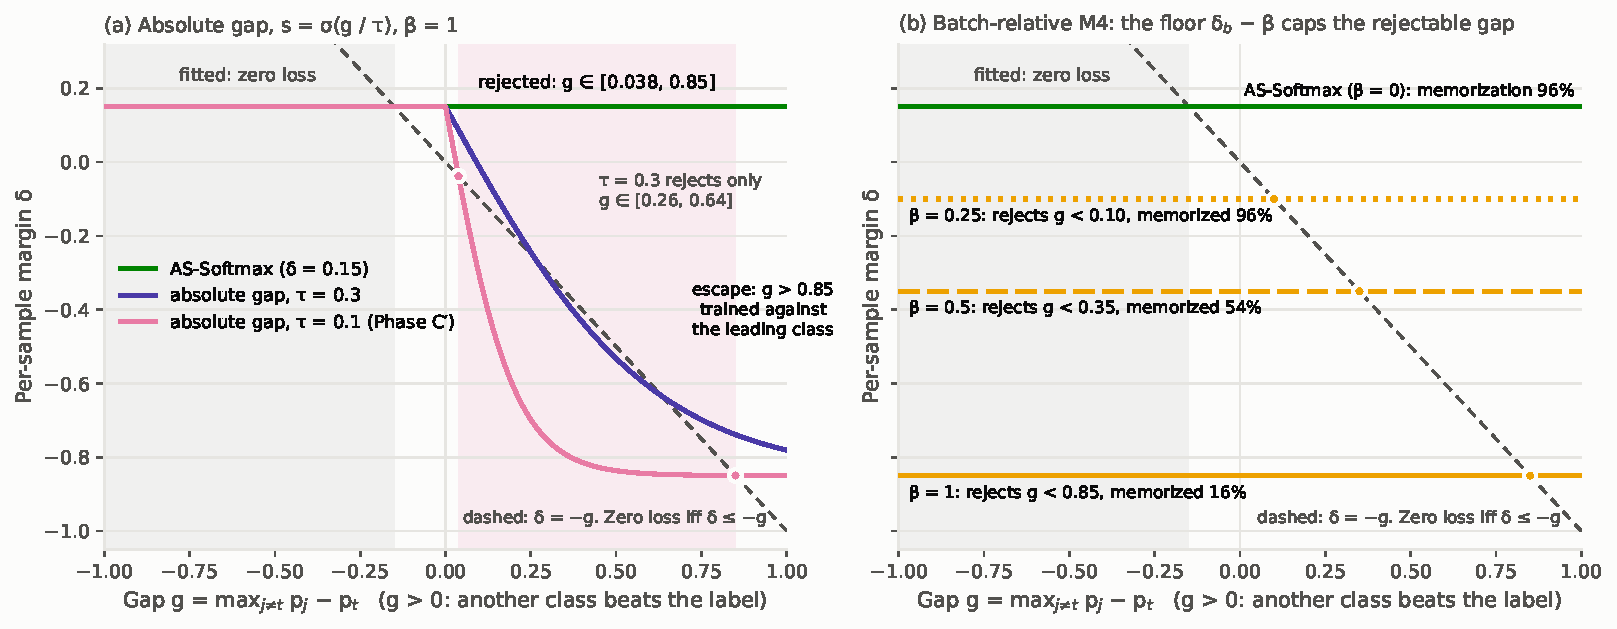
\includegraphics[width=\linewidth]{figures/fig1_geometry.pdf}
  \caption{Margin geometry. A sample has zero loss iff its margin lies on or below the dashed
  line $\delta = -g$ (\cref{prop:zero}). (a)~The absolute-gap margin rejects a fixed band of gaps,
  $[0.038, 0.85]$ at $\tau = 0.1$ and only $[0.26, 0.64]$ at $\tau = 0.3$, independent of the noise
  rate (\cref{cor:band}). Above $g_{\mathrm{hi}}$ the sample escapes rejection. (b)~The batch-relative
  margin can reach no lower than $\dbase - \beta$, so it can only reject gaps below $\beta - \dbase$
  (\cref{prop:reject}). The memorization figures are from \cref{tab:main} (40\% symmetric noise,
  last epoch).}
  \label{fig:geometry}
\end{figure}

\subsection{Batch-relative statistics are blind to the noise rate}

\begin{proposition}[Affine invariance]
\label{prop:blind}
Let $s_i = h(z_i)$ for an increasing function $h$ of the batch z-score $z_i$ of $p_{y,i}$. Replacing every
$p_{y,i}$ in the batch by $a\,p_{y,i} + b$ with $a > 0$ leaves every $s_i$ unchanged. The fraction
of the batch with $s_i \ge h(k)$, $k > 0$, is at most $1/(1+k^2)$, and the fraction with
$z_i > 0$ is the fraction below the batch mean, whatever the share of wrong labels in the batch.
\end{proposition}

A batch with 40\% wrong labels and a clean batch at an earlier stage of training can have the same
standardized distribution of $p_y$, and then receive the same suspicion scores. The statistic
measures \emph{relative} fit only. It flags roughly the lower half of every batch, and how much of
that half is rejected is set by $\beta$ through \cref{prop:reject}, not by the data. The method
therefore carries a fixed rejection rate that nobody chose explicitly. It suits one noise level
and over- or under-rejects everywhere else. On clean data it discards correctly labeled samples
that are merely below average (\cref{sec:results}). Small-loss selection has the same
blindness by construction. There the rate is an explicit input $r$, typically set to the true
noise rate, which is information the method should not need.

\subsection{An absolute statistic gives a rate-free rejection band}

\begin{corollary}[Rejection band]
\label{cor:band}
With $s_i = \sigma(g_i / \tau)$ and full strength $\beta$, the rejected gaps are
\[
  R = \{\, g > 0 : \beta \tanh\!\big(g / 2\tau\big) \ge \dbase + g \,\},
\]
an interval $[g_{\mathrm{lo}}, g_{\mathrm{hi}}]$ (possibly empty) that depends on
$(\beta, \tau, \dbase)$ alone. For $\beta = 1$, $\dbase = 0.15$:
$R = [0.038, 0.850]$ at $\tau = 0.1$ and $R = [0.265, 0.635]$ at $\tau = 0.3$.
\end{corollary}

The band involves neither the batch, nor the noise rate, nor an estimate of either. What the rule
rejects follows the data: on clean data, once the model fits, few samples have $g > 0$ and few are
rejected; under heavy noise, many are. The rule is rate-free, not parameter-free. Its three
constants fix the band in advance, and \cref{fig:geometry}a shows that the scale matters: at
$\tau = 0.3$ the band shrinks to $[0.26, 0.64]$, the most contradicted labels escape, and
memorization stays at the level of plain AS-Softmax (96\%, \cref{tab:main}). The absolute rule
trains on two regions: near-ties, $g \in (-\dceil, g_{\mathrm{lo}})$, and the escape region
$g > g_{\mathrm{hi}}$.

\subsection{AS-Softmax and memorization}

\begin{observation}
\label{obs:as}
Cross-entropy gives every sample a logit gradient of $\ell_1$-norm $2(1 - p_y) > 0$. AS-Softmax
gives exactly zero to every fitted sample, $g \le -\dbase$. As clean samples become fitted, a larger
share of each update comes from the samples that are not, and once early learning is over most of
those carry wrong labels. Adam's per-coordinate normalization \citep{kingma2015adam,loshchilov2019adamw} makes
the step size largely insensitive to the overall gradient scale. We therefore expect AS-Softmax to
memorize corrupted labels faster than cross-entropy in mid-training, with both saturating
eventually.
\end{observation}

The observation is a prediction, not a theorem. \Cref{sec:mechanism} measures both the
memorization curves and the share of gradient carried by mislabeled samples.

\section{Experimental protocol}
\label{sec:setup}

\paragraph{Pre-registration.}
The study ran in phases. Before each phase we wrote down its hypotheses, numeric pass criteria and
the decision each outcome would trigger, in a dated plan kept in the repository history
(\cref{app:prereg}). Phase~A replicated an earlier two-seed result on five seeds. Phase~B compared
against GCE, SCE and small-loss selection; it failed as specified. Phase~B$'$ removed two
confounds named before it ran, and Phase~C added noise types, noise rates, the strength sweep and
the realistic selection protocol. Phase~C$'$ tested the two self-calibrating statistics. Its rule
read: if neither passes at its home condition, 40\% symmetric noise, write the result up as a
reframing and do not proceed to the planned real-noise benchmark. That is what happened, and this
paper is the write-up. No method or hyperparameter was changed after its test results were seen.
One design change was made before launch on a training-set diagnostic that involved no test
accuracy (\cref{app:mixture}).

\paragraph{Data and noise.}
20~Newsgroups \citep{lang1995newsweeder} with headers, footers and quotes removed, and empty
documents dropped: 11{,}014 training and 7{,}317 test documents in 20 classes. We hold out 10\% of
the training set (1{,}101 documents) \emph{with its noisy labels} as the model-selection set and
train on the remaining 9{,}913. Test labels are never corrupted. \emph{Symmetric} noise at rate
$\eta$ replaces each training label, independently with probability $\eta$, by a class drawn
uniformly from the 19 others. \emph{Pair-flip} noise \citep{han2018coteaching} replaces it by
$(y + 1) \bmod 20$, a systematic confusion the model can learn as a pattern. Conditions: symmetric
$\eta \in \{0, 0.2, 0.4, 0.6\}$ and pair-flip $\eta \in \{0.2, 0.4\}$. The corruption is drawn once
per condition and shared by every method and seed.

\paragraph{Model and training.}
\texttt{bert-base-uncased} \citep{devlin2019bert} with mean pooling and a linear head, inputs
truncated to 128 tokens, dropout 0.1. AdamW \citep{loshchilov2019adamw} at a constant learning
rate of $2\times10^{-5}$, weight decay 0.01, batch size 16, gradient clipping at 1.0, 8 epochs
(4{,}960 steps), full precision. Seeds 42--46 vary the head's initialization, dropout and batch
order.

\paragraph{Model selection and metrics.}
Each run reports three test accuracies: \textbf{sel}, at the epoch with the highest accuracy on the
noisy held-out labels (earliest on ties), our headline; \textbf{final}, at the last epoch, which is
what training without any validation set yields; and \textbf{best}, at the epoch with the highest
\emph{clean test} accuracy, an oracle upper bound reported only for completeness.
\textbf{Memorization} is measured on a fixed probe of 1{,}200 training examples, shared by all
methods. Of the probe's corrupted examples (477 at 40\% symmetric noise), it is the fraction the
model predicts as its corrupted label at the last epoch.

\paragraph{Methods.}
\begin{itemize}
  \item \textbf{CE}: cross-entropy.
  \item \textbf{GCE} \citep{zhang2018gce}: $q = 0.7$; $q = 0.4$ in the tuning grid.
  \item \textbf{SCE} \citep{wang2019sce}: $(\alpha, \beta) = (0.1, 1)$, $A = -4$; $(1, 1)$ in the grid.
  \item \textbf{Small-loss}: single-network small-loss selection, i.e.\ Co-teaching's selection
  rule without the second network \citep{han2018coteaching}. The forget rate ramps linearly to $r$
  over the first 30\% of training, with $r = \eta$ (the \emph{true} noise rate, an oracle) and
  $r = \eta/2$ in the grid.
  \item \textbf{AS-Softmax} \citep{lv2023assoftmax}: $\delta = 0.15$ with a 10\% linear warm-up.
  \item \textbf{M4 (batch-relative)}: \cref{def:family} with the batch z-score, $T = 1$,
  $\beta \in \{0.25, 0.5, 1\}$ ($\beta = 1$ unless stated).
  \item \textbf{M4 absolute gap}: $\tau = 0.1$, $\beta = 1$; $\tau = 0.3$ as the one pre-registered
  scale alternative.
  \item \textbf{M4 loss mixture}: \cref{app:mixture}.
\end{itemize}
Every suspicion margin uses $\dbase = \dceil = 0.15$, floor $-1$, and the 0~$\to$~30\% ramp of
$\beta$. The ramp matches small-loss's schedule, a confound identified and removed in Phase~B$'$.
Baselines received the tuning grid above, evaluated with noisy-held-out selection at 40\%
symmetric noise. The grid changed GCE and SCE by less than 0.15 points. For small-loss,
$r = \eta/2$ scored higher than the oracle rate (66.75 vs.\ 65.61, $t = 1.2$, \cref{tab:main}).
The grid ran only at 40\% symmetric noise, so the multi-condition comparisons use the default
settings listed first.

\paragraph{Statistics.}
We report mean $\pm$ standard deviation over the five seeds, and paired differences between
methods over the same seeds with the paired $t$ statistic (4 degrees of freedom; $|t| > 2.78$
corresponds to $p < 0.05$, two-sided). With five seeds we call a difference \emph{established} only
past that threshold. A run takes about 11 minutes on one RTX 3080~Ti; the study used about 280.

\section{Results}
\label{sec:results}

\subsection{The home condition: 40\% symmetric noise}

\begin{table}[t]
\centering
\caption{40\% symmetric noise, all fourteen methods (5 seeds, mean $\pm$ sd). \textbf{sel}: test
accuracy at the epoch chosen on noisy held-out labels (headline). \textbf{final}: last epoch.
\textbf{best}: oracle epoch chosen on the clean test set. \textbf{mem}: corrupted probe labels
predicted as given at the last epoch. $\Delta$CE: paired sel difference to cross-entropy, with $t$.}
\label{tab:main}
\small
\renewcommand{\arraystretch}{0.95}
\begin{tabular}{llccccc}
\toprule
& method & sel & final & best (oracle) & mem & $\Delta$CE sel ($t$) \\
\midrule
\multirow{7}{*}{\rotatebox{90}{baselines}}
& CE                              & 66.97\sd{0.48} & 51.51\sd{1.22} & 67.08\sd{0.50} & 96.1 & --- \\
& GCE, $q=0.7$                    & 67.34\sd{0.78} & 65.55\sd{0.86} & 67.80\sd{0.34} & 24.3 & $+0.36$ (0.7) \\
& GCE, $q=0.4$                    & 67.20\sd{0.60} & 57.51\sd{1.41} & 67.62\sd{0.45} & 60.6 & $+0.23$ (0.6) \\
& SCE, $(0.1, 1)$                 & 66.64\sd{0.88} & 63.07\sd{0.75} & 67.69\sd{0.28} & 29.1 & $-0.33$ ($-0.7$) \\
& SCE, $(1, 1)$                   & 66.73\sd{0.69} & 54.62\sd{1.16} & 67.50\sd{0.56} & 75.6 & $-0.24$ ($-0.6$) \\
& small-loss, $r = \eta$ (oracle) & 65.61\sd{1.19} & 64.38\sd{0.94} & 67.10\sd{0.33} & 25.9 & $-1.37$ ($-2.3$) \\
& small-loss, $r = \eta/2$        & 66.75\sd{1.13} & 58.70\sd{0.63} & 67.11\sd{0.57} & 58.2 & $-0.22$ ($-0.5$) \\
\midrule
\multirow{4}{*}{\rotatebox{90}{\scriptsize batch-rel.}}
& AS-Softmax ($\beta = 0$)        & 66.71\sd{0.91} & 53.42\sd{0.64} & 67.40\sd{0.47} & 96.4 & $-0.26$ ($-0.7$) \\
& M4, $\beta = 0.25$              & 66.74\sd{0.99} & 53.04\sd{2.74} & 67.43\sd{0.54} & 96.0 & $-0.24$ ($-0.4$) \\
& M4, $\beta = 0.5$               & 66.84\sd{0.63} & 58.49\sd{1.47} & 67.19\sd{0.54} & 53.8 & $-0.14$ ($-0.5$) \\
& M4, $\beta = 1$                 & \textbf{67.44}\sd{0.55} & \textbf{66.72}\sd{0.80} & 67.64\sd{0.28} & 16.1 & $+0.47$ (1.4) \\
\midrule
\multirow{3}{*}{\rotatebox{90}{\scriptsize self-calib.}}
& absolute gap, $\tau = 0.1$      & 66.39\sd{0.65} & 65.93\sd{1.01} & 67.01\sd{0.44} & \textbf{9.5} & $-0.59$ ($-1.8$) \\
& absolute gap, $\tau = 0.3$      & 66.56\sd{1.15} & 52.58\sd{1.57} & 67.23\sd{0.49} & 95.6 & $-0.41$ ($-0.8$) \\
& loss mixture                    & 65.33\sd{0.90} & 64.55\sd{0.34} & 66.26\sd{0.53} & 23.1 & $-1.64$ ($-3.0$) \\
\bottomrule
\end{tabular}
\end{table}

\Cref{tab:main} gives the condition the batch-relative margin was designed around. Four
observations stand out.

\emph{Model selection on noisy labels compresses everything.} Under sel, twelve of the fourteen
methods fall within 0.8 points of CE, and none is established as better than CE. Early stopping on
noisy held-out labels already captures most of what robust training buys at this noise rate. The
differences reappear without selection: at the last epoch CE has dropped to 51.5\%, and the two
rejection margins hold 66.7\% (batch-relative) and 65.9\% (absolute), above GCE (65.6) and
small-loss (64.4).

\emph{The absolute margin memorizes least.} It ends training having fitted 9.5\% of the
corrupted probe labels. That is the lowest of all fourteen methods, against 24--26\% for GCE and
oracle small-loss and 96\% for CE. It does so without being told the noise rate.

\emph{The strength sweep is a threshold, as \cref{prop:reject} predicts.} Memorization goes
96 / 96 / 54 / 16\% for $\beta = 0 / 0.25 / 0.5 / 1$. The cap $\beta - \dbase$ explains the shape.
At $\beta = 0.25$ only gaps below 0.10 are rejectable, while the mislabeled samples' gaps are
large once early learning has happened. The same geometry predicts the failure of the
absolute gap at $\tau = 0.3$. Its band $[0.26, 0.64]$ lets the most contradicted labels escape,
and it memorizes like AS-Softmax (95.6\%).

\emph{Estimating the rate is not enough.} The loss-mixture statistic estimates the noise rate well
(0.35 $\pm$ 0.01 against a true 0.40) but is the least accurate margin, 1.64 points below CE
($t = -3.0$). It also memorizes more than the absolute rule (23\% vs.\ 9.5\%). Knowing \emph{how
many} labels are wrong did not tell it \emph{which}.

\subsection{Across noise conditions}

\begin{table}[t]
\centering
\caption{All six conditions for the five main methods (5 seeds, mean $\pm$ sd). Top: test accuracy
with noisy-held-out selection. Middle: last epoch. Bottom: memorization of corrupted labels at the
last epoch (\%). Small-loss equals CE at $\eta = 0$ ($r = 0$). Small-loss is given the true rate.}
\label{tab:conditions}
\small
\setlength{\tabcolsep}{4.5pt}
\begin{tabular}{lcccccc}
\toprule
& \multicolumn{4}{c}{symmetric} & \multicolumn{2}{c}{pair-flip} \\
\cmidrule(lr){2-5}\cmidrule(lr){6-7}
method & 0\% & 20\% & 40\% & 60\% & 20\% & 40\% \\
\midrule
\multicolumn{7}{l}{\emph{sel (noisy held-out selection)}} \\
CE              & \textbf{71.38}\sd{0.61} & 68.34\sd{0.80} & 66.97\sd{0.48} & 63.65\sd{0.99} & 67.39\sd{1.48} & 57.31\sd{4.79} \\
small-loss      & \textbf{71.38}\sd{0.61} & 68.72\sd{0.83} & 65.61\sd{1.19} & 63.41\sd{1.24} & 67.62\sd{0.64} & 59.42\sd{2.35} \\
GCE             & 71.15\sd{0.39} & \textbf{68.86}\sd{0.27} & 67.34\sd{0.78} & \textbf{64.55}\sd{0.51} & \textbf{68.16}\sd{0.52} & 57.76\sd{6.15} \\
M4 (batch-rel.) & 67.55\sd{1.27} & 68.49\sd{0.51} & \textbf{67.44}\sd{0.55} & 62.52\sd{1.37} & 66.93\sd{0.66} & 52.71\sd{3.65} \\
absolute gap    & 69.88\sd{0.37} & 67.83\sd{0.66} & 66.39\sd{0.65} & 63.27\sd{1.03} & 68.04\sd{0.52} & \textbf{62.69}\sd{1.55} \\
\midrule
\multicolumn{7}{l}{\emph{final (last epoch)}} \\
CE              & \textbf{71.25}\sd{0.14} & 62.94\sd{0.68} & 51.51\sd{1.22} & 36.89\sd{1.57} & 61.96\sd{1.37} & 48.95\sd{1.39} \\
small-loss      & \textbf{71.25}\sd{0.14} & 67.39\sd{0.91} & 64.38\sd{0.94} & 61.99\sd{0.39} & 65.33\sd{0.87} & 53.63\sd{2.61} \\
GCE             & 70.85\sd{0.52} & \textbf{68.91}\sd{0.33} & 65.55\sd{0.86} & 57.24\sd{0.60} & \textbf{67.35}\sd{0.78} & 49.32\sd{0.71} \\
M4 (batch-rel.) & 64.43\sd{2.25} & 68.51\sd{0.55} & \textbf{66.72}\sd{0.80} & 54.92\sd{2.07} & 64.98\sd{0.70} & 47.19\sd{1.85} \\
absolute gap    & 68.75\sd{0.89} & 67.60\sd{0.90} & 65.93\sd{1.01} & \textbf{62.38}\sd{1.55} & 66.43\sd{1.18} & \textbf{56.44}\sd{5.13} \\
\midrule
\multicolumn{7}{l}{\emph{memorization at the last epoch (\%)}} \\
CE              & --- & 93.5 & 96.1 & 97.4 & 96.6 & 97.1 \\
small-loss      & --- & 29.4 & 25.9 & 13.4 & 50.9 & 48.5 \\
GCE             & --- & 16.1 & 24.3 & 31.4 & 39.3 & 80.4 \\
M4 (batch-rel.) & --- & \textbf{7.0} & 16.1 & 32.6 & 34.3 & 66.5 \\
absolute gap    & --- & 9.3 & \textbf{9.5} & \textbf{8.0} & \textbf{17.5} & \textbf{26.3} \\
\bottomrule
\end{tabular}
\end{table}

\begin{figure}[t]
  \centering
  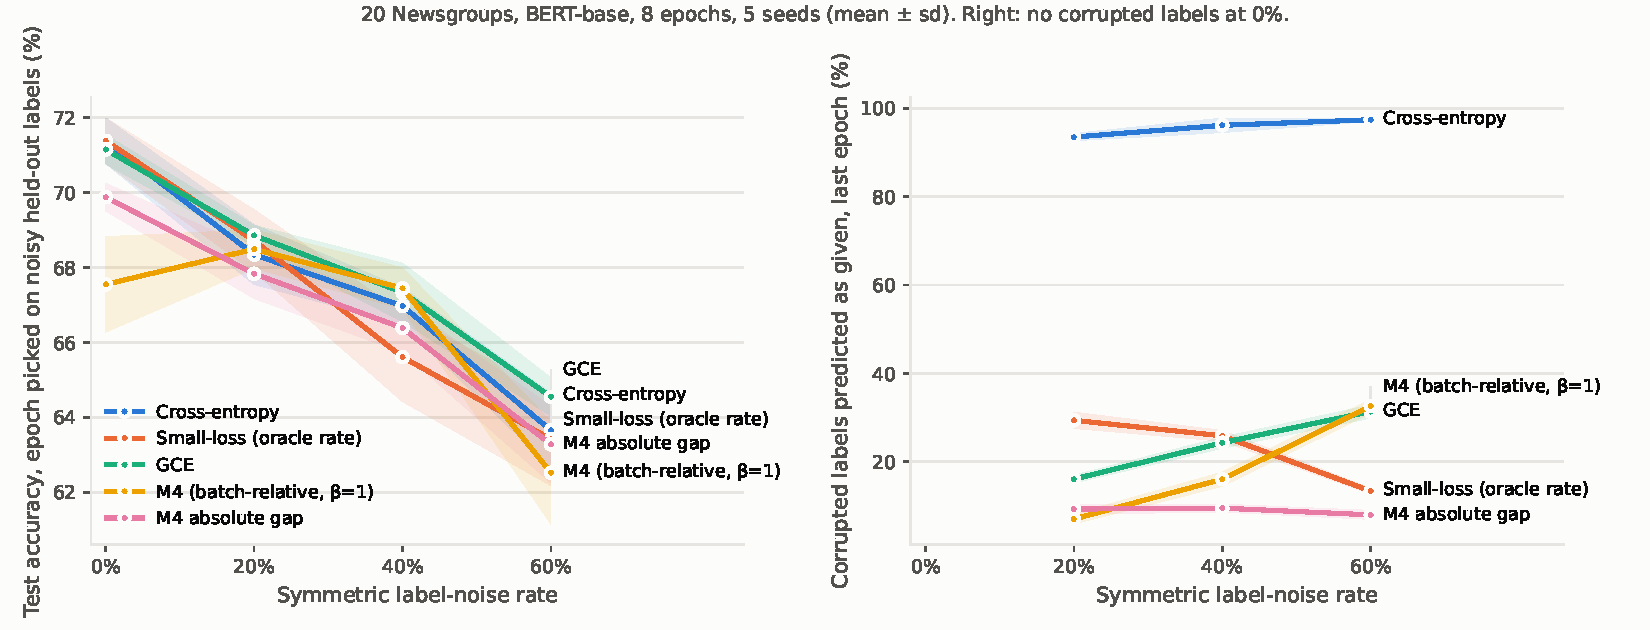
\includegraphics[width=\linewidth]{figures/figC1_noise_curves.pdf}
  \caption{Symmetric noise. Left: test accuracy with noisy-held-out selection. Right: memorization
  of corrupted labels at the last epoch. Mean $\pm$ sd over 5 seeds. The batch-relative margin
  (yellow) is competitive only near 40\%, the rate its fixed strength suits. The absolute margin
  (pink) keeps memorization at 8--10\% at every rate.}
  \label{fig:noise}
\end{figure}

\begin{figure}[t]
  \centering
  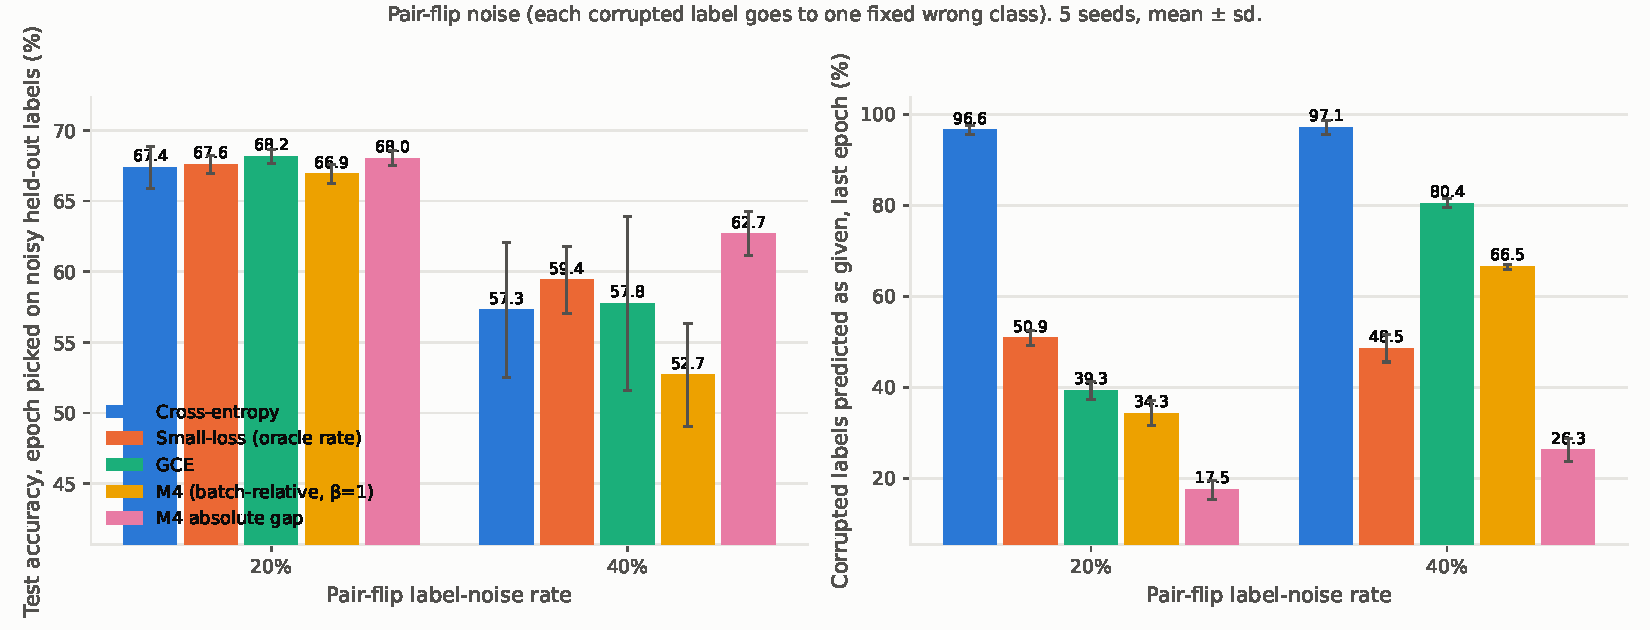
\includegraphics[width=\linewidth]{figures/figC2_pair_noise.pdf}
  \caption{Pair-flip noise, where each corrupted label goes to one fixed wrong class. The absolute
  margin is the only method whose accuracy holds at 40\% and the only one that keeps memorization
  well below half.}
  \label{fig:pair}
\end{figure}

\Cref{tab:conditions} and \cref{fig:noise,fig:pair} test the two statistics' predictions away
from the home condition.

\emph{The batch-relative margin is noise-blind, as \cref{prop:blind} predicts.} On clean data it
loses 3.83 points to CE (5/5 seeds, $t = -5.2$), and 6.8 at the last epoch: it keeps discarding
correctly labeled samples that are merely below their batch's average. At 60\% symmetric noise it
under-rejects (memorization 33\%, twice its 40\% level) and trails GCE by 2.0 points ($t = -3.4$).
Under 40\% pair-flip noise it is the worst method, 4.6 points below CE ($t = -2.0$) and 6.7 below
small-loss ($t = -3.6$). The strength that suits 40\% symmetric noise is a hidden rejection rate
that suits nothing else.

\emph{The absolute margin follows the data, but pays on easy regimes.} Its clean-data cost falls
from 3.83 to 1.51 points; that is still established ($t = -5.1$), so P1 fails. Under structured
noise it is the best method: at 40\% pair-flip it reaches 62.69, $+5.38$ over CE ($t = 3.4$, 5/5
seeds) and $+3.27$ over small-loss given the true rate ($t = 3.3$). It is $+4.93$ over GCE, though
GCE's variance across seeds is too large to establish that ($t = 1.7$). Its memorization there
(26\%) is half of small-loss's and a third of GCE's. On symmetric noise it trails GCE by 1.0
($\eta = 0.2$, $t = -3.4$), 0.95 ($\eta = 0.4$, $t = -1.9$) and 1.3 points ($\eta = 0.6$,
$t = -2.1$). The rule rejects every sample the model currently disagrees with. That includes hard
but correctly labeled samples, and on easy regimes GCE's soft down-weighting is the better trade.

\emph{Without a validation set, the absolute margin's advantage grows with the noise.} At the last
epoch its difference to GCE goes from $-2.1$ (clean) and $-1.3$ (20\%) to $+0.4$ (40\%),
$+5.1$ (60\%, $t = 9.7$, 5/5 seeds) and $+7.1$ (pair 40\%, $t = 3.1$). Under symmetric noise the
absolute margin loses at most 0.9 points between the selected and the last epoch (GCE: up to 7.3),
because it keeps refusing to fit what it disagrees with. Under pair-flip noise both decay more
(absolute gap 6.3, GCE 8.4 points at 40\%).

\subsection{Pre-registered verdicts}

\begin{table}[t]
\centering
\caption{Pre-registered criteria (fixed before the corresponding runs) and outcomes. Accuracies
use sel unless noted. N1--N4 were defined for the batch-relative M4 (Phases A--C), P1--P4 for the
self-calibrating statistics (Phase C$'$). The loss mixture was eliminated at P3 and, by the
pre-registered rule, not run elsewhere.}
\label{tab:verdicts}
\small
\begin{tabular}{p{0.24\linewidth}p{0.42\linewidth}p{0.24\linewidth}}
\toprule
criterion & outcome & verdict \\
\midrule
N1 replicate (4 ep., final) & M4 $-$ CE $= +1.81$, $t = 4.4$, 5/5 seeds; memorization 17\% vs.\ 35\% & pass \\
N2 $\ge$ small-loss $-$ 0.5 & 4 ep.\ final: $-0.39$ after removing the timing confound (B$'$); 8 ep.\ sel: $+1.84$ & pass \\
N3 $\ge \max$(GCE, SCE) & 4 ep.\ final: $-0.49$ vs.\ GCE; 8 ep.\ sel: $+0.11$ & fail at 4 ep., tie at 8 \\
N4 memorization falls steadily in $\beta$ & 96 / 96 / 54 / 16\%: monotone, threshold-shaped (\cref{prop:reject}) & partial \\
\midrule
P1 clean cost $\ge$ CE $-$ 0.5 & absolute gap $-1.51$ ($t = -5.1$) & fail \\
P2 adaptivity & masked-slot ratio flat (0.996) at every rate; mixture estimate 0.35 at $\eta = 0.4$ & fail as worded \\
P3 home $\ge$ best baseline $-$ 0.5 $= 66.84$ & absolute gap 66.39; mixture 65.33 & fail (both) \\
P4 pair 40\%: $\ge$ CE, within 2 of small-loss & absolute gap 62.69 vs.\ 57.31 / 59.42 & pass \\
\bottomrule
\end{tabular}
\end{table}

\Cref{tab:verdicts} collects the pre-registered tests. The decisive one is P3. The bar was the best
tuned baseline at the home condition minus half a point, $67.34 - 0.5 = 66.84$, and neither
self-calibrating statistic reached it. By the rule we fixed in advance, the absolute-gap margin is
therefore not presented as a new method, and the real-noise benchmark (CIFAR-10N/100N,
\citealp{wei2022cifarn}) was not run. P2 failed for a reason we only understood afterwards. Its
measure, the fraction of masked non-target slots, is dominated by AS-Softmax's masking of fitted
samples (0.996 for every method in the family at every noise rate), so it cannot register sample-level
adaptivity. The sample-level evidence is the flat 8--10\% memorization across symmetric noise rates
in \cref{tab:conditions}, against small-loss's 29\% $\to$ 13\%. We report P2 as failed, as worded.

\subsection{Mechanism}
\label{sec:mechanism}

\begin{figure}[t]
  \centering
  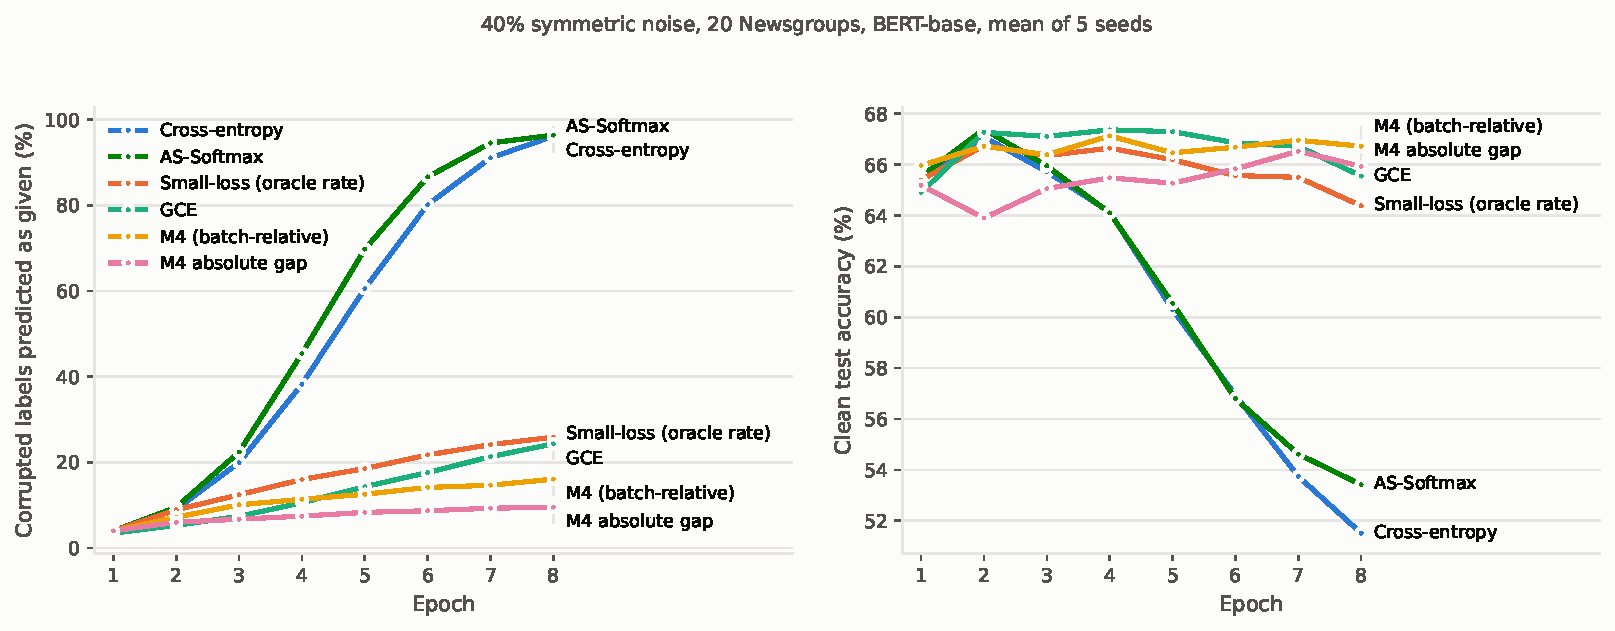
\includegraphics[width=\linewidth]{figures/fig4_dynamics.pdf}
  \caption{40\% symmetric noise, per epoch, mean of 5 seeds. Left: memorization of corrupted labels.
  AS-Softmax (green) memorizes faster than cross-entropy at epochs 3--7, on every seed. Right: clean
  test accuracy, the degradation that noisy-held-out selection has to catch.}
  \label{fig:dynamics}
\end{figure}

\paragraph{AS-Softmax memorizes faster than cross-entropy.}
\Cref{obs:as} predicts that zeroing the gradient of fitted samples shifts each update toward the
unfitted, mostly mislabeled ones. \Cref{fig:dynamics} confirms the prediction. AS-Softmax's
memorization exceeds CE's at epochs 3 through 7 on all five seeds: by 2.5 points at epoch 3
($t = 3.5$), 7.2 at epoch 4 ($t = 5.5$), 9.2 at epoch 5 ($t = 13.0$), 6.5 at epoch 6 and 3.5 at
epoch 7. Both saturate at 96\% by epoch 8. The same holds in the earlier 4-epoch runs (39.4\% vs.\
34.7\% at the last epoch). On its own, the base loss of the margin family is \emph{less}
noise-robust than cross-entropy. As a base for rejection it is nonetheless the better choice. In a
Phase~B$'$ control with identical rejection decisions, training the kept samples with CE instead of
AS-Softmax cost 4.1 points (63.3 vs.\ 67.4, 4 epochs, \cref{app:prereg}). We have not isolated why.

\paragraph{Where the gradient goes.}
\TODO{Fill from \texttt{runs/mechanism/summary.md} once the 42 instrumented runs finish (3 seeds;
the instrumentation reproduces Phase~C's accuracies exactly). Report, at the last epoch of 40\%
symmetric noise: the share of gradient carried by mislabeled probe samples for CE / AS / M4 /
absolute gap / small-loss / GCE; the fraction of mislabeled samples rejected (zero gradient with
$g > 0$); the fraction of clean samples with zero gradient at 0\% noise for M4 vs.\ absolute gap
(the clean-cost mechanism of \cref{prop:blind}); and the share of the mislabeled samples' gradient
in the escape region $g \ge 0.8$ (\cref{prop:reject}). Insert \texttt{fig5\_mechanism.pdf}.}

\section{Discussion}
\label{sec:discussion}

\paragraph{What the margin view buys.}
Writing rejection as a margin did not produce a method that beats GCE on symmetric noise. It did
make three properties of selection rules visible before any training run, and each was then
measured. First, \emph{relative} statistics carry a hidden rate. A z-score, a rank or a fixed
budget rejects the same share of a clean batch as of a corrupted one (\cref{prop:blind}). That
is why the batch-relative margin wins exactly at one noise level and why small-loss needs the
oracle rate. Second, an \emph{absolute} statistic turns the rejection threshold into a constant of
the loss, a band of label gaps (\cref{cor:band}). The rejected share then follows the data,
including structured noise, where rate-based selection has no reason to pick the right samples.
Third, any margin family with a floor has an \emph{escape region} (\cref{prop:reject}). It
explains the threshold-shaped strength sweep and the failure of the wider-temperature variant.
It also identifies a defect of our recipe: the most confidently contradicted labels receive a
near-maximal gradient toward the wrong class. The remedy is $\beta \ge 1 + \dbase$, which makes
the band reach $g = 1$; with $\beta = 1.15$, $\tau = 0.1$ it becomes $[0.032, 1.0)$. We did not
run it, because the pre-registered protocol froze $\beta$ before Phase~C$'$, and we leave it as a
stated prediction.

\paragraph{When to reject and when to down-weight.}
The absolute rule discards every sample the model currently disagrees with. Under symmetric noise
many of those are hard but correct, and GCE, which only down-weights them, is 0.9--1.3 points
better. Under pair-flip noise, disagreement is the better signal. A fixed wrong class is learned
as a pattern, so mislabeled samples do not stand out by loss rank (small-loss memorizes half of
them). They appear to stand out by disagreement before the pattern is learned (the absolute rule
memorizes a quarter).
The same contrast appears without model selection. The heavier or more structured the noise, the
larger the absolute rule's last-epoch lead over GCE: $+5.1$ at 60\% symmetric and $+7.1$ at 40\%
pair-flip.

\paragraph{Limitations.}
One dataset, one model, one modality, and synthetic noise only. The real-noise benchmark was cut
by our own pre-registered rule, so the claims above are about 20~Newsgroups with injected noise.
Five seeds resolve differences of about one point at best: several comparisons we describe
($+4.9$ over GCE under pair-flip, $-0.95$ at 40\% symmetric) are not established at $p < 0.05$.
Small-loss is the single-network rule, not Co-teaching's two networks, and DivideMix-style
semi-supervised pipelines are out of scope, since they are training procedures rather than losses.
The baselines' tuning grid ran only at 40\% symmetric noise. Training was fixed at 8 epochs with a
constant learning rate. The suspicion margins inherit AS-Softmax's base margin, which we showed
memorizes faster than CE on its own.

\section{Conclusion}
\label{sec:conclusion}

In masked softmax, a sample's loss vanishes exactly when its label gap reaches the negative of its
margin. A negative margin is therefore sample rejection, and the choice of selection rule becomes
the choice of a margin function. The view makes falsifiable predictions, and they held in a
pre-registered study. Relative statistics are noise-blind. An absolute ``another class beats the
label'' statistic rejects a fixed, rate-free band of gaps, memorizes the fewest corrupted labels and
is the most robust rule under structured noise. A margin floor leaves an escape region that
shapes how the rule responds to its strength. The absolute rule did not clear our bar against GCE
on clean and symmetric noise, and we report it as a unifying account with measured consequences,
not as a new state of the art.


\bibliographystyle{plainnat}
\bibliography{refs}

\appendix
\section{Proofs}
\label{app:proofs}

\paragraph{\Cref{prop:zero}.}
Every $j \ne y$ is dropped iff $p_y - p_j \ge \delta$ for all $j \ne y$, i.e.\ iff
$\min_{j\ne y}(p_y - p_j) = -g \ge \delta$. Then $K_\delta = \{y\}$ and
$\ell_\delta = -o_y + \log e^{o_y} = 0$. Because the mask is under stop-gradient it is held fixed
when differentiating, and the loss is identically zero as a function of $o$, so
$\nabla_o \ell_\delta = 0$. Otherwise $K_\delta \supsetneq \{y\}$. Writing $\tilde p$ for the
softmax restricted to $K_\delta$, $\ell_\delta = -\log \tilde p_y > 0$ and
$\partial \ell_\delta / \partial o_y = \tilde p_y - 1 \ne 0$. Finally,
$p_y - p_{j^\star} = -g < \delta$, so $j^\star \in K_\delta$. \hfill$\square$

\paragraph{\Cref{cor:selection}.}
$\delta = -1$ gives $-g \ge -1 = \delta$ for every sample, so by \cref{prop:zero} the loss and
gradient vanish. $\delta = 1$ keeps every $j$ with $p_j > p_y - 1$, which is every class unless
$p_y = 1$ exactly, so $\ell_1$ is cross-entropy. The batch mean then averages over all $B$ samples
rather than the kept ones, a constant factor per batch. \hfill$\square$

\paragraph{\Cref{prop:reject}.}
Write $u = \dbase - \beta(2s - 1)$, so $\delta = \min(\max(u, -1), \dceil)$. By
\cref{prop:zero} the loss vanishes iff $\delta \le -g$. A minimum is $\le -g$ iff one of its
arguments is: either $\dceil \le -g$ (fitted), or $\max(u, -1) \le -g$. Since $g < 1$ we have
$-1 < -g$, so the latter holds iff $u \le -g$, i.e.\ $\beta(2s - 1) \ge \dbase + g$. For the
escape region, $2s - 1 < 1$ gives $\beta(2s - 1) < \beta \le \dbase + g$ whenever
$g \ge \beta - \dbase$. Such a sample is not fitted either, since $g > 0 \ge -\dceil$ (for
$\beta > \dbase \ge 0$). By \cref{prop:zero} it then trains against $j^\star$. For the absolute
statistic and $g > g_{\mathrm{hi}}$, $\delta \to \dbase - \beta = -0.85$, and the only class
that can satisfy $p_j > p_y + 0.85$ is $j^\star$, so $K_\delta = \{y, j^\star\}$. \hfill$\square$

\paragraph{\Cref{prop:blind}.}
The batch mean and standard deviation of $a p + b$ are $a\bar p + b$ and $a\,\mathrm{sd}(p)$, so
every $z_i$ and hence every $s_i = h(z_i)$ is unchanged. The empirical distribution of $z$ has mean
0 and variance 1, and Cantelli's inequality bounds the fraction with $z \ge k$ by $1/(1+k^2)$.
For increasing $h$, $s_i \ge h(k) \iff z_i \ge k$. \hfill$\square$

\paragraph{\Cref{cor:band}.}
With $s = \sigma(g/\tau)$, $2\sigma(x) - 1 = \tanh(x/2)$. By \cref{prop:reject} a sample with
$g > 0$ is rejected iff $f(g) = \beta\tanh(g/2\tau) - g - \dbase \ge 0$. On $g \ge 0$, $\tanh$ is
concave, so $f$ is concave and its superlevel set $\{f \ge 0\}$ is an interval, possibly empty. The
endpoints quoted in the text are computed on a grid of $2\times10^5$ points
(\texttt{AbsoluteGapMargin.rejection\_band}). \texttt{tests/test\_mechanism.py} checks that the
implemented loss has zero gradient exactly on this set, and positive gradient elsewhere, for
$\tau \in \{0.1, 0.3\}$. \hfill$\square$

\section{The loss-mixture statistic}
\label{app:mixture}

The loss-mixture statistic keeps a per-sample exponential moving average (momentum 0.5) of
$-\log p_y$ over the steps at which each training example is seen. Every 100 steps, once half the
training set has been seen, it fits one- and two-component Gaussian mixtures (20 EM iterations) to
the \emph{log} of these averages. The mixture is \emph{active} only if BIC prefers two components
and the high component's mean loss is at least $\log C$, the loss of a uniform prediction. When
inactive, $s_i = 1/2$ for every sample and the loss is exactly AS-Softmax. When active, $s_i$ is
the posterior of the high-loss component, and that component's weight is logged as an estimate of
the noise rate. This is the selection statistic of DivideMix \citep{li2020dividemix} expressed as a
margin.

\paragraph{Design iteration before launch.}
The first design fitted raw losses and gated on BIC alone. A diagnostic on the training set with
ground-truth flip labels (one CE epoch at 40\% symmetric noise; no test accuracy involved) showed
two problems. Raw-loss fits over-estimated the rate (0.59 at a true 0.40, precision 0.67), while log
fits gave 0.39--0.40 with precision 0.82--0.87 and AUC 0.94--0.96. And on \emph{clean} data BIC
still preferred two components, with weight 0.44--0.52, because not-yet-fitted clean samples form
a second mode. A rejected sample is never fitted, so that error would lock in. The two modes differ
in location: mislabeled samples sat at a loss of about 3.5, above $\log 20 \approx 3.0$, while the
unfitted clean mode was at 1.5 and falling. The chance-level anchor follows from that and is not a
tuned threshold. In the main runs the mixture estimated the rate at $0.35 \pm 0.01$ (true 0.40) yet
trained worse than the absolute rule (\cref{tab:main}).

\section{Pre-registration record and earlier phases}
\label{app:prereg}

The plan document and every decision rule live in the repository, timestamped by its version
history. The negative-margin idea came out of an earlier, failed project on class-pair-structured
margins for AS-Softmax. There, one two-seed run at 40\% symmetric noise first showed the
batch-relative margin memorizing about a quarter as many corrupted labels as CE. Phase~A was
pre-registered to re-test that result on five seeds before anything was built on it.
\Cref{tab:phases} lists every phase and \cref{tab:phaseab} the 4-epoch results of Phases A--B$'$.

\begin{table}[h]
\centering
\caption{Phases, the decision fixed before each, and the outcome.}
\label{tab:phases}
\small
\begin{tabular}{p{0.13\linewidth}p{0.42\linewidth}p{0.37\linewidth}}
\toprule
phase & fixed in advance & outcome \\
\midrule
A & 5 seeds, 4 epochs, final epoch: M4 must memorize less than CE on every seed and beat it by
$> 2$ sd; else stop & pass: $+1.81$ ($t = 4.4$), memorization 17\% vs.\ 35\% \\
B & M4 $\ge$ small-loss $- 0.5$ and $\ge \max$(GCE, SCE) & fail: GCE / small-loss / SCE all
$+1.7$ to $+2.3$ ahead \\
B$'$ & two named confounds (rejection timing; AS vs.\ CE base); one variant each; stop if the
better is $> 1$ pt below small-loss & timing fixed: 67.41 vs.\ 67.80 (tie); CE base: 63.29 \\
C & noise types and rates, $\beta$ sweep, 8 epochs, noisy-held-out selection & best at sym 40\%;
fails clean ($-3.8$) and pair 40\% ($-4.6$); noise-blindness diagnosed \\
C$'$ & two self-calibrating statistics, P1--P4 (\cref{tab:verdicts}); P3 failure $\Rightarrow$
reframing write-up, no CIFAR-N & P3 fails for both; P4 passes for the absolute gap \\
E & instrumented re-runs (3 seeds, no new method or setting) for \cref{sec:mechanism} &
\TODO{fill} \\
\bottomrule
\end{tabular}
\end{table}

\begin{table}[h]
\centering
\caption{Phases A--B$'$: 40\% symmetric noise, 4 epochs, clean-test selection (\emph{best}) and
last epoch (\emph{final}), 5 seeds. ``M4, delayed'' is the original schedule (rejection off for
the first 30\% of training, full strength only at the end); ``M4, matched'' uses small-loss's
schedule; ``M4, CE base'' makes the same rejection decisions as ``matched'' but trains kept
samples with CE.}
\label{tab:phaseab}
\small
\begin{tabular}{lccc}
\toprule
method & best & final & mem @final (\%) \\
\midrule
CE                  & 67.46\sd{0.48} & 63.84\sd{0.50} & 34.7 \\
AS-Softmax          & 67.70\sd{0.60} & 64.32\sd{0.40} & 39.4 \\
GCE                 & 68.28\sd{0.22} & 67.90\sd{0.53} & 9.3 \\
SCE                 & 68.18\sd{0.87} & 67.38\sd{0.54} & 9.1 \\
small-loss (oracle) & 68.09\sd{0.24} & 67.80\sd{0.27} & 12.4 \\
M4, delayed         & 67.94\sd{0.34} & 65.65\sd{0.91} & 17.2 \\
M4, $\beta = 0.5$, delayed & 67.89\sd{0.42} & 64.68\sd{0.47} & 34.5 \\
M4, matched         & 68.05\sd{0.53} & 67.41\sd{0.60} & 8.1 \\
M4, CE base         & 65.29\sd{0.82} & 63.29\sd{0.95} & 12.4 \\
\bottomrule
\end{tabular}
\end{table}

\section{Reproducibility}
\label{app:repro}

Every run is one command, \texttt{python experiments/run.py --config <yaml>}, with the seed, noise
rate and noise type as overrides. The configurations are in \texttt{configs/phase\_c/} (Phases C,
C$'$) and \texttt{configs/final/} (Phases A--B$'$). The drivers \texttt{experiments/phase\_c.py} and
\texttt{experiments/mechanism.py} run the sweeps and rebuild the summary tables. Figures come from
\texttt{experiments/make\_paper\_figures.py}. The 115 unit tests (\texttt{python -m pytest tests/})
include the closed-form checks of \cref{sec:theory}. Hardware: one RTX 3080~Ti (12\,GB), about
11 minutes per 8-epoch run.


\end{document}
